
Let $U_{1},U_{2}\sim\mathcal{U}(0, 1)$ be independently distributed random variables and let $f_{1}, f_{2}:\mathbb{reals}\rightarrow\mathbb{R}$ be measurable functions. Let $\mathcal{Q}$ the distribution of $(f_{1}(X_{1}), f_{2}(X_{2}))$ on $[0, 1]^{2}$.

Let us consider the functions $f_{1}(x) = (1 + \cos(\pi x)) / 2$, $f_{2}(x) = \sin(\pi x)$, $x\in\mathbb{R}$. Let $S$ be the set defined as 
\begin{align*}
	S = \{(x_{1}, x_{2})\in\mathbb{R}^{2}:\|(x_{1}-\frac{1}{2}, x_{2}-\frac{1}{2})\|_{1}\leq\frac{1}{4}\}.
\end{align*}

\begin{figure}
  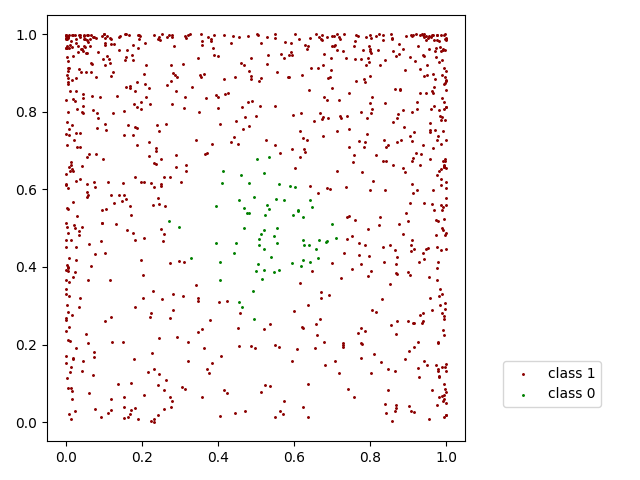
\includegraphics[scale=0.8]{./images/training_data}
  \caption{Training dataset consisting of 1000 samples.}
\end{figure}

Now, for training consider a randomly sampled training set of size $N=1000$, and for $n=m=6$, consider equidistant partitions of the intervals $[0, 1]$. We evaluate the performance of the trained classifier using the metrics \textit{accuracy (acc)}, \textit{true positive rate (tpr)} and \textit{false negative rate (fnr)}.  Using a randomly sampled evaluation dataset consisting of $1500$ samples we get 
\begin{align*}
	acc = 0.956, ~ tpr = 0.9835, ~ fpr = 0.0165.
\end{align*}





